\documentclass[DIV=12,headings=normal,pdftex,headinclude=false,footinclude=false,final]{scrreprt}
\usepackage{spreadtab}
\usepackage{xspace}
\usepackage[ngerman]{babel}
\usepackage{tocbasic}
\usepackage{graphicx}
%\usepackage[linkcolor=black,colorlinks=true,urlcolor=gray,breaklinks=true]{hyperref}
\usepackage{scrlayer-scrpage}
\usepackage{longtable}
\usepackage{caption}
\usepackage{float}
\usepackage{xcolor}
\usepackage{colortbl}
\usepackage[utf8]{inputenc}
\usepackage[T1]{fontenc}
\usepackage{wrapfig}

\usepackage{listings}
\usepackage{xcolor}

%\usepackage{arial}
\usepackage{ragged2e}

\usepackage{parcolumns}

%urls and breaking them correctly
\usepackage[hyphens]{url}
\usepackage{xurl}
\PassOptionsToPackage{hyphens}{url}\usepackage[citecolor=blue,linkcolor=black,colorlinks=true,urlcolor=gray,breaklinks=true]{hyperref}

%for displaying code correctly
\definecolor{codegreen}{rgb}{0,0.6,0}
\definecolor{codegray}{rgb}{0.5,0.5,0.5}
\definecolor{codepurple}{rgb}{0.58,0,0.82}
\definecolor{backcolour}{rgb}{0.96,0.96,0.96}

\lstdefinestyle{mystyle}{
    backgroundcolor= \color{backcolour},   
    commentstyle= \color{codegreen},
    keywordstyle= \color{blue},
    numberstyle= \tiny\color{codegray},
    stringstyle= \color{codepurple},
    basicstyle= \ttfamily\footnotesize,
    breakatwhitespace=false,         
    breaklines=true,                 
    captionpos=b,                    
    keepspaces=true,                 
    numbers=left,                    
    numbersep=5pt,                  
    showspaces=false,                
    showstringspaces=false,
    showtabs=false,                  
    tabsize=2
}
\lstset{style=mystyle}


\graphicspath{{./}{./Images/}}

\setlength\headheight{1.75cm}
\ihead{\small{G. Hauschild, K. Wilfert StuArb IT-Security 2020/21}}
\chead{}
\ohead{
\includegraphics[height=0.05\textheight]{fh_logo}}
\pagestyle{scrheadings}


\titlehead{
\includegraphics[width=5cm]{fh_logo}}
\title{Studienarbeit über die Schwachstelle\\CVE-2017-0144\\''EternalBlue''}
\subtitle{IT-Sicherheit\\Wintersemester 2020/2021}
\author{Georg Hauschild (00175118) und Kay Wilfert (01642116)}
\date{\today
\\
\textbf{Zusammenfassung}
\\
\justify
Im Rahmen der Wahlkurses IT-Sicherheit wurde die Sicherheitlücke, welche im März 2017 mit dem Beinamen EternalBlue bekannt wurde, auf ihre inneren Vorgänge untersucht.
Von der NSA für verdeckte Ermittlungen benutzt, stellte Sie für viele Windows-Versionen
aufgrund der dort integrierten SMBv1 Schnittstelle eine Bedrohung dar. Es wird näher untersucht, welche Bugs ausgenutzt werden, um über das SMB-Protokoll eine Remote Code Execution zu bewirken.
}


\begin{document}
\maketitle

\pagenumbering{roman}

\tableofcontents

\listoffigures

\chapter*{Abkürzungsverzeichnis}

\noindent
\textbf{CIFS}: Common Internet File System\\
Urversion des SMB, Begriff in frühen Versionen austauschbar\\

\noindent
\textbf{CVE}: Common Vulnerabilities and Exposures\\
Liste von Schwachstellen und Sicherheitslücken, jede eindeutig mittels eines CVE-Codes identifizierbar\\

\noindent
\textbf{FEA}: File Extension Attributes\\
Dateisystemfunktion für nicht vom Dateisystem berücksichtige Datei-Metadaten\\

\noindent
\textbf{MBR}: Master Boot Record\\
Enthält notwendiges Startprogramm für verschiedene OS, sowie Partitionstabelle.\\

\noindent
\textbf{MFT}: Master File Table\\
Master File Table, enthält Informationen über abgelegte Dateien auf NTFS Datenträgern\\

\noindent
\textbf{NAS(-Server)} Network Accessible Storage (Server)\\
Im lokalen Netzwerk erreichbarer Server, der Dateien und Verzeichnisse für Teilnehmer zur Verfügung stellt\\

\noindent
\textbf{RCE}: Remote Code Execution\\
Eine Attacke, bei der Angreifer Schadcode auf entfernten Rechnern ausführen\\

\noindent
\textbf{SMB(v1)}: Server Message Block (Version 1)\\
Netzwerkprotokoll zum Austausch von Dateien und Services im Netzwerk\\

\noindent
\textbf{TCP}: Transmission Control Protocol\\
Protokoll zum Datenaustausch im Netzwerk über aufgebaute Verbindung\\

\noindent
\textbf{UDP}: User Datagram Protocol\\
Protokoll zur Datenübermittlung ohne zuvor aufgebaute Verbindung\\

\noindent
\textbf{HAL}: Hardware Abstraction Layer\\
Zwischen Windows Betriebssystem und Hardware vermittelnde Abstraktionsschicht\\

\noindent
\textbf{IPC\$}: Inter Process Communication Share\\
Auch Null Session Connection; Lässt anonyme Verbindungen auf SMB Server zu\\

\newpage
\pagenumbering{arabic}


\chapter{Vorwort}
Da Microsofts Implementierung des SMB Protokolls deren geistiges Eigentum ist, muss sich an die Nutzungsbedingungen gehalten werden. Deshalb muss eingeräumt werden, dass es sich bei den in der Studienarbeit vorkommenden Codefragmenten um Code aus Online-Quellen handelt und keine Treiber für die Studienarbeit dekompiliert wurden \cite{MS:LicTerm}. Weiterhin gibt es viele verschiedene Skripte, die im Laufe der Zeit auf unterschiedliche Art und Weise die Kern-Programmierfehler ausnutzen, die zur RCE führen, besonders beim Grooming des Speichers Auch unterscheidet sich die Erfolgswahrscheinlichkeit und Methode stark je nach Windowsversion und Exploittechniken der Skripte. Deshalb liegen Crashes der angegriffenen Maschine in der Natur des Exploits. Resultat eines Angriffs ist somit entweder Remote Code Execution oder Denial of Service. Weiterhin liegt der Fokus der Studienarbeit auf dem Kern von EternalBlue, um dem Leser die generellen Programmierfehler und deren Bedeutung näher zu bringen. 


\chapter{EternalBlue Malware}
In vielerlei Hinsicht ist die Entstehungsgeschichte des EternalBlue Exploits eng mit der US-amerikanischen National Security Agency verbunden. Eine Unterabteilung der Agency, zum damaligen Zeitpunkt als ''Tailored Access Operations'' bekannt \cite{CS}, untersuchte über ein Jahr lang das Windows Betriebssystem auf Schwächen, die der Agency beim Zugriff auf fremde Systeme helfen könnten\cite{WP}. Letzten Endes wurden mehrere Sicherheitslücken im SMB Protokoll der Windows Plattform gefunden, die es ermöglichten, mittels eines speziell angefertigten Paketes einen Rechner zu kapern und auf ihm beliebigen Code auszuführen \cite{Avast}.
Eigens für die Sicherheitslücke, die später als CVE-2017-0144 veröffentlicht wurde, programmierte die Agency das Hacking-Tool EternalBlue, so benannt nach der Tendenz, die angegriffenen Rechner zu crashen, was einen Bluescreen als Folge hatte. Das Hacking Tool zählte intern zur NOBUS-Gruppe (Nobody but us), da eine solche Sicherheitslücke aufgrund der enormen Konsequenzen nie an die Öffentlichkeit gelangen sollte \cite{CS}. Dieses Vorgehen, Zero-Day-Exploits zu sammeln und zu Waffen umzufunktionieren sorgte schon damals in einigen NSA Officials für Unbehagen, was, wie sich herausstellte, eine berechtigte Kritik war \cite{WP}.
Jedoch kam es genau zu einem solchen Ernstfall, als die Hackergruppe der ''Shadow Brokers'' im August 2016 die gesamte Familie der SMB-Schwachstellen zusammen mit dem Hacking Tool in einem Leak, der als ''Lost in Translation'' bezeichnet wurde \cite{Medium:ExpBible}, veröffentlichte. Somit waren auch Amateure fähig, die Lücke zu nutzen, um Schaden anzurichten. Die NSA reagierte zunächst lediglich mit einer Benachrichtigung an Microsoft aber klärte die Öffentlichkeit nicht bezüglich der enormen Gefahr, die von dem Leak ausging, auf \cite{WP}.

\begin{figure}[H]
    \centering
    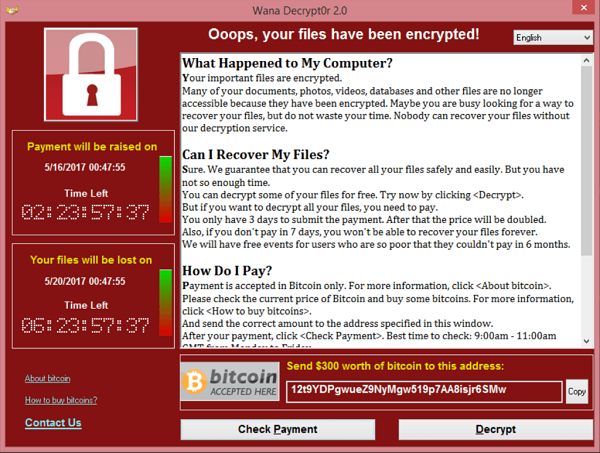
\includegraphics[width=10cm]{wanna_decrypt0r_2.0.png}
    \caption[WannaDecryptor Screenshot (SecureList) URL: \url{securelist.com/wannacry-ransomware-used-in-widespread-attacks-all-over-the-world/78351/}]{Ein Screenshot des  WannaDecryptor 2.0 Virus}
    \label{img:wanna_decrypt0r}
\end{figure}

\noindent
Am 12. Mai 2017 wurde das gewaltige Gefahrenpotenzial dann realisiert. Ein Ransomware-Virus namens WannaCrypt, auch bekannt unter einigen Aliasnamen, nutze den modifizierten EternalBlue Code zum Infizieren und Verschlüsseln von Windows-PCs auf der ganzen Welt \cite{Avast}. Zwar veröffentlichte Microsoft schon zwei Tage nach Ausbruch ein Sicherheitsupdate, was aber erst nach und nach von Nutzern installiert werden musste \cite{MSSB}. Deshalb wurden die persönlichen Daten unzähliger Nutzer auf deren Rechnern verschlüsselt und der Zugriff dauerhaft gesperrt. Zu sehen war wie bei jeder Ransomeware nur eine Lösegeldforderung und das Versprechen, die Daten durch eine Zahlung, zum Beispiel in Bitcoin, wieder herzustellen. Sonst würden die Daten gelöscht werden. Das Virus verbreitete sich mit einer Geschwindigkeit von circa 10.000 Neuinfektionen pro Stunde, sodass nach dem ersten Tag bereits 230.000 Windows-Maschinen in über 150 Ländern betroffen waren. Dabei schienen die Attacken wahllos verschiedene Ziele anzugreifen, wodurch keine spezifische Taktik erkennbar war. Es folgte ein enormer monetärer Schaden in der Höhe von ungefähr vier Milliarden US-Dollar, wobei ein genauer Betrag aufgrund der hohen Dunkelziffer schwer einzuschätzen und nicht bekannt ist, wie viele Personen auf die Drohung reagierten \cite{Avast}.

\begin{figure}[H]
    \centering
    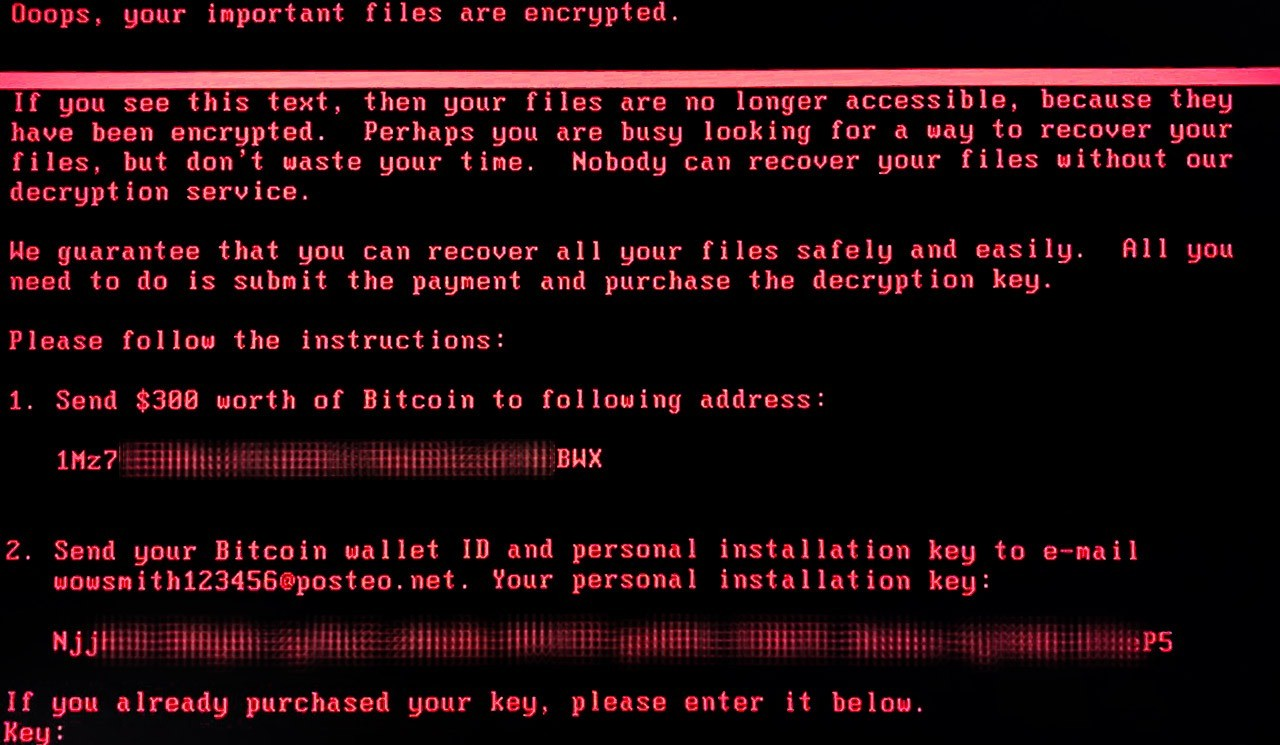
\includegraphics[width=10cm]{notpetya_ransomware.jpg}
    \caption[NotPetya Screenshot, Nutzer ''GrEat'' (Kaspersky), URL: \url{https://media.kasperskydaily.com/wp-content/uploads/sites/92/2017/06/27133735/wannamore-ransomware-screenshot.jpg}]{Screenshot einer Variante des WannaCry Virus}
    \label{img:not_petya}
\end{figure}

\noindent
Als noch verheerender erwies sich der NotPetya Virus, eine mit dem EternalBlue-Kern aufgerüstete Version eines bereits im Vorjahr umgehenden, weniger bekannten und weitaus weniger schädlichen Virus am 16.6.2017. NotPetra zeichnete sich dadurch aus, dass sowohl MBR als auch MFT verschlüsselt worden sind, was eine Wiederherstellung der Daten unmöglich machte, auch wenn der Sperrbildschirm dies gegen 300 USD versprach. Der durch diese zweite gigantische Ransomware-Welle verursachte Schaden wurde auf etwa 10 Milliarden USD geschätzt, wobei der Datenverlust und die Menschenleben, die durch lahmgelegte Rechner in Krankenhäusern und öffentlichen Einrichtungen in Gefahr gebracht worden sind, nicht mit eingerechnet sind \cite{Avast}.\\
Wie sich nach Analyse der Malware heruasstellte besaß keiner der beiden Viren, insbesondere wie oben beschrieben NotPetya, die nötige Infrastruktur auf, um nach dem Zahlen des Lösegelds in Bitcoin das Entschlüsseln der Daten wieder zu ermöglichen. Das lässt darauf schließen, dass nicht monetäere Gewinn, sondern Schaden das Hauptziel der Hacker war \cite{Sil}.

\noindent
Microsoft reagiere im Angesicht des entstandenen Schadens und des Mangels an Vorsicht der US-Regierung mit einer Warnung, dass der Trend, Zero-Days zu sammeln, um Sie für digitale Kriegsführung zu nutzen ein gefährliches Unterfangen sei. Es wurde zu Verhandlungen für eine digitale Genfer Konvention aufgerufen und ein Entwurf vorgelegt, der einen groben Plan skizziere, keine Repertoire an Sicherheitlücken anzulegen und Cyberkriegsführung zu regulieren \cite{MS:EB}.

\chapter{Grundlagen}
Dieses Kapitel beleuchtet die inneren Vorgänge des Server Message Blocks 1.0 und die Fehler, die das erfolgreiche Ausführen eines RCE Angriffs auf Windows Hosts ermöglichen. Die National Vulnerability Database bewertete diese Sicherheitslücke in CVSS Version mit 8.1 von maximal zehn Punkten \cite{NVD} als schwerwiegend. Zweifelsohne aufgrund der sehr hohen Verbreitung der Verwundbarkeit und des Schweregrads eines Hacking-Angriffs. \\
Um den Exploit besser verstehen zu können, müssen vorab einige grundlegende Begriffe erklärt werden, die für die Durchführung einer solchen Hacking Attacke essenziell sind.

\section{Das SMB Protokoll}\label{sec:SMB}
Das im schon mehrere Dekaden alte Application-Layer-Netzwerk-Protokoll\cite{Medium} wurde von 1983 von Barry Feigenbaum (IBM) 1983 vorgestellt und fand später erstmals in Windows 95 Verwendung. Das in der damiligen Forrm als CIFS bekannte Protokoll dient seitdem auf jeder Windows Plattform bis heute dem Austausch über Netzwerkressourcen wie Dateien, Verzeichnisse, Drucker und Programmierschnittstellen \cite{CompWeek:SMB}. Spätere Server Message Block Iterationen wurden dann stets mit Versionsnummern versehen. Anfangs baute CIFS Verbindungen über ein weiteres Protokoll namens NetBIOS over TCP auf, das die UDP Ports 137 für Namensauflösung, 138 für Paketübermittlung und TCP-Port 139 für Verbindungsaufbau und Datenübertragung nutzte \cite{MS:NetBIOS}. Dieses wurde allerdings schon ab Windows 2000 von regulären TCP-Verbindungen auf Port 445 und dem DNS-Protokoll abgelöst \cite{IONOS}. Die davor meist als CIFS bezeichnete Urversion der unter Windows implementierten Schnittstelle wird von hier an im Rest der Arbeit als SMBv1 bezeichnet. Weiterhin wird es sich stets um die Version des Protokolls über TCP auf Port 445 handeln.\\
Trotz der engen Assoziation mit Windows handelt es sich jedoch um ein plattform- und dateiformatunabhängiges Protokoll, das via Samba Shareware auch auf Linux angewendet werden kann\cite{IONOS}.\\
SMBv1 Packets bestehen aus drei Teilen: einem 32Bytle langem Header, einem Parameter- und einem Datenblock, wobei der Header stets dasselbe Format besitzt aber Parameter und Datenblock sich je nach Format unterscheiden \cite{MS:CIFS_MSG}.

\section{File Extended Attributes}\label{sec:FEA}
File Extended Attributes sind Datenstrukturen, die erweiterte Metadaten beherbergen, die nicht relevant für das System sind. Darin können zum Beispiel der Autor, das Encoding einer Textdatei oder andere Informationen gespeichert werden \cite{Wiki:FEA}. Solche zusätzlichen Informationen werden im SMBv1 Protokoll in FEA Strukturen gespeichert, die die Form von Key-Value-Paaren annehmen, welche wiederum in Listen abgespeichert werden \cite{CP}. SMB ist ein plattformübergreifendes Protokoll, welches demnach auch für mehrere Dateisysteme besagte Listenstrukturen implementiert haben muss \cite{CompWeek:SMB}. Darunter fallen auch Microsofts WindowsNT und IBMs OS/2 Betriebssystem, welches seit Windows NT in allen weitern Windowsversionen als Subsystem integriert ist \cite{MS:OS2Subsys}. Die FEA-Formate und deren Listenstrukturen für beide Betriebssysteme sind essenziell für das Gelingen des Exploits.

\section{Non-paged Memory Pool und HAL}\label{sec:mempool}
Zur Verwaltung des Arbeitsspeicherressourcen besitzt Windows einen Memory Manager. Dieser hat als Aufgabe, für Prozesse und deren Verwaltung Arbeitsspeicher zu reservieren und wieder danach wieder frei zu geben \cite{Medium:ExpBible}. Der Memory Manager schöpft bei dieser Verwaltung Speicherbereiche aus dem für das System reservierten Arbeitsspeicher, der bereits für den virtuellen Adressraum gemappt wurde. Unterteilt wird hierbei in zwei sogenannte Memory Pools, in denen Memoryblöcke allokiert werden: Den paged und den non-paged Memory Pool \cite{MS:MemPools}. Die zusätzliche Abstraktionschicht des Mappens von virtuellen auf physikalische Speicheradressen ermöglicht unter anderem dieses Paging. Als Paging bezeichnet man hierbei das Ein- und Auslagern von Arbeitsspeicherblöcken ins Dateisystem, um in Ausnahmefällen mehr Speicher zur Verfügung zu haben als physikalisch verbaut \cite{CompWeek:Paging}. Beim non-paged Pool, der besonders bei Treibern Gebrauch findet, ist dies nicht der Fall. Im non-paged Memory Pool finden deshalb die meisten Speichermanipulationen statt, da in ihm durch die beiden Treiber svr.sys und srvnet.sys, respektive die Treiber der Protokolle SMBv1 und SMBv2, Speicherbereiche reserviert, frei gegeben und gelesen werden, die zum Platzieren und Laden des Schadcodes dienen \cite{SS:EB}.

\section{Der IPC Share}\label{sec:IPC}
Um ohne entsprechende Credentials eine Verbindung zum integrierten SMBv1 Server einer Windows Maschine zu aufzubauen, ist ein Inter Process Communication Share nötig. Auch als Null-Session bekannt, erlauben sie das anonyme Anmelden ohne Username oder Passwort, sowie beschränkten Zugriff auf Serverfunktionen wie zum Beispiel das Erstellen von Named Pipes \cite{MS:IPC}. Durch das Verwenden solcher benannten Pipes kann über Netzwerk und mehrere Instanzen hinweg vollduplex kommuniziert werden, der Client seine Identität wechseln und Prozesse können ihre eigenen Berechtigungen verwalten \cite{MS:NP}. Das Aufbauen einer SMB Session erfolgt über eine durch den IPC\$ Share ermöglichte anonyme Anmeldung und eine solche Named Pipe.


\section{Grooming}\label{sec:Grooming}
Durch die Technik des Heap Grooming kann dafür gesorgt werden, dass zwei kontrollierbare Speicherblöcke mit hoher Wahrscheinlichkeit nebeneinander allokiert werden. Das gilt bei EternalBlue als Voraussetzung für den Speicherzugriff auf anliegende Chunks durch einen Overflow in einem vorhergehenden Speicherbereich. Es gibt mehrere Methoden, das für EternalBlue umzusetzen. Zum Beispiel kann durch das Öffnen mehrerer großer simulatener Transaktionen mit dem Server ein ganzer zusammenhängender Speicherbereich reserviert werden, sofern die finalen der Transaktion zugehörigen Packages  noch nicht gesendet wurden\cite{}. Lücken können durch Senden des letzten Packages und somit dem Schließen Transaktion, was den Speicher wieder deallokiert, ermöglicht werden. Somit wird neu allokierter Speicher mit hoher Wahrscheinlichkeit zwischen die bereist bestehenden Blöcke allokiert.\\ Zusätzlich kann der verfügbare Speicher durch die unter Punkt \ref{sec:MemAlloc} beschriebene Methode verkleinert werden, indem vor den Transaktionen große Bereiche belegt werden.


\chapter{Der EternalBlue Exploit}
Der Exploit nutzt mehrere Fehler im SMBv1 Netzwerkprotokoll aus, wodurch Remote Code Execution auf verwundbaren Windows Maschinen ermöglicht wird.\\ Hierfür werden SMB Instruktionen zusammengestellt, die den Arbeitsspeicher geschickt so manipulieren, dass mehrere Fehler im Protokoll zusammenspielen, um Schadcode zu platzieren und ihn durch speicherübergreifende Zugriffe zu triggern\cite{Medium}. Bei der Exploit Speichermanipulation kommt auch der HAL Heap zum Einsatz. Dies hat zum Vorteil, dass unter vielen Windows-Arten der Speicheradressbereich bekannt ist \cite{GH:FEA}. Besonders wichtig und komplex ist der erste in einer Reihe von Bugs, der für den Zweck dieser Studienarbeit unter die Lupe genommen wird.

\section{Fehler beim Casten einer FEA Liste}\label{sec:FEA_Cast}
Da einer der Hauptzwecke des SMB Protokolls der Austausch von Dateien ist, müssen auch die mit den Files assoziierten Metadaten korrekt zwischen File- und Betriebssystemen gecastet werden können. Diese FEAs werden in Listenstrukturen innerhalb des Protokolls festgehalten und beim Handling von Dateien je nach Bedarf von einem ins andere Format konvertiert. Hierbei wurde ein Bug entdeckt, der beim Casten einer OS/2 FEA Liste in eine WindowsNT FEA Liste entsteht \cite{TM:EB}. Die relevanten FEA Strukturen und Listen entsprechen dem folgendem Code:\\

\begin{lstlisting}[language=C,caption={Die zwei relevanten FEAs und exemplarisch die NTFEA-Liste\cite{CP}},captionpos=b]
/**
 * Single OS/2 Fea Entry
 */
struct Os2Fea{
    //Flags
    UCHAR ExtendedAttributeFlag;
    //Length of AttriubuteName Field
    UCHAR AttributeNameLengthInBytes;
    //Length of AttriubuteName Field
    USHORT AttributeNameValueLengthInBytes;
    //Extended attribute name
    UCHAR AttributeName[AttributeNameLengthInBytes + 1];
    //Extended attribute value
    UCHAR AttributeValue[AttributeValueLengthInBytes]; 
}
 
/**
 * OS/2 List Structure
 */
struct Os2FeaList{
    //The total size of the FeaRecords +4 Bytes
    ULONG SizeOfListInBytes; 
    //The total size of the FeaRecords +4 Bytes
    UChar Os2FeaRecords;
}
 
/**
 * Windows NT List Structure
 */
struct NtFeaList{
    //Offset to the next NtFea record of NtFeaList type
    ULONG NextEntryOffset;
    //Flags
    UCHAR Flags;
    UCHAR NtFeaNameLength;
    USHORT NtFeaValueLength;
    CHAR NtFeaName[NtFeaNameLength];
    CHAR NtFeaValue[NtFeaValueLength];
}
\end{lstlisting}

\noindent
Durch Ausnutzen dieses Konvertierungsfehlers wird ein Bufferoverflow im non-paged Kernel Pool Heap erzeugt. Dabei nimmt die Funktion SrvOs2FeaListToNt eine Os2 FEA Liste entgegen und ruft SrvOs2FeaListSizeToNt auf, was die richtige Größe für das Resultat der Konvertierung berechnen soll, um anschließend  einen entsprechend großen Buffer im non-paged Kernel Pool zu allokieren. Hierfür iteriert die Funktion durch die Liste der FEAs und ruft für jedes Listenelement die Methode SrvOs2FeaToNt auf, was für jedes FEA die größe im NT-Format berechnet und in der variable akkumuliert zur NT-Liste hinzugefügt \cite{TM:EB}. Das Ergebnis wird dann in einer Variablen in Os2FeaList, genannt SizeOfListInBytes, durch Überschreiben des vorherigen Wertes gespeichert. Jedoch werden alle Elemente vorher auf Validität überprüft und die SizeOfListInBytes entsprechend so angepasst, dass ungültige FEAs abgezogen werden. Gibt es keine ungültigen FEAs, bleibt die Variable unberührt. SizeOfListInBytes ist auch nicht die SMB Paketgröße beschränkt, da die FEAs langer Listen lediglich auf Pakete aufgeteilt werden. Erst beim ankommen des letzten Packets mit FEA Daten wird der Bug getriggert\cite{CP}.

\begin{figure}[H]
    \centering
    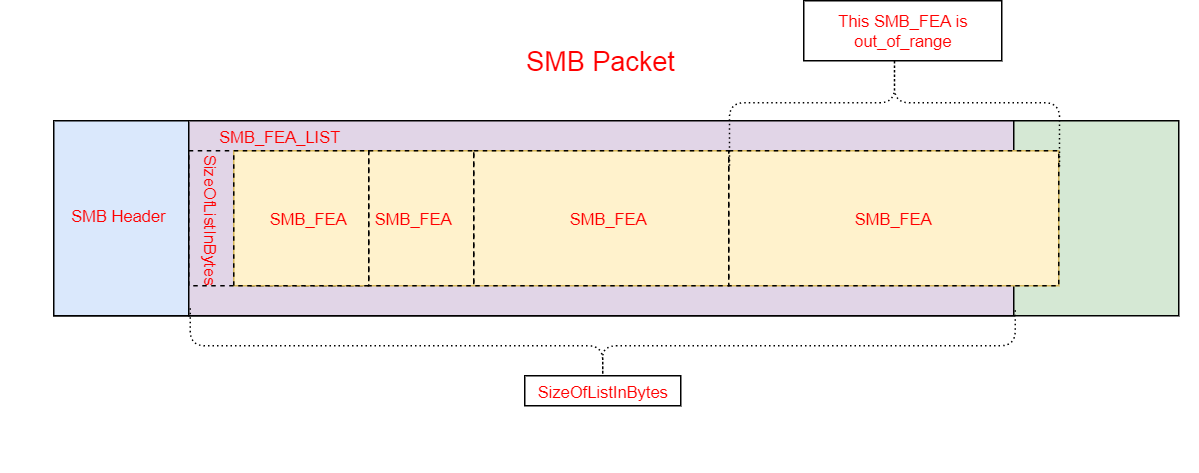
\includegraphics[width=15cm]{checkpoint_before_shrink.png}
    \caption[FEAList vor Verkleinerung, Nadav Grossmann (Checkpoint Research),URL: \url{https://research.checkpoint.com/wp-content/uploads/2017/09/eternalblue4.png}]{Speicherbelegung der FEA Liste vor Verkleinerung}
    \label{img:fealist_before_shrinking}
\end{figure}

\noindent
Wird zum Zweck der Berechnung der Listengröße der OS/2 Liste für die Konvertierung zu einer NT FEA Liste die SMB Funktion SrvOS2FeaListSizeToNt mit einem Pointer zum Beginn der OS/2 FEA Liste aufgerufen, so wird durch die FEAs iteriert und die Größe der einzelnen Einträge zu einem Pointer hinzugezählt \cite{TM:EB}.
Anschließend wird, um die tatsächliche Listengröße zu kalkulieren, der 32 Bit Endpointer vom 32 Bit Startpointer abgezogen und die Differenz, als 16 Bit WORD SizeOfListInBytes zugewiesen \cite{Scad:EB}.
Dabei wird die 32 Bit (DWORD) große Variable, die die ursprüngliche Listenlänge in Bytes festhält fälschlicherweise als 16 Bit (WORD) Variable gecastet. Da ein WORD und ein DWORD sich per Definition um 2 Byte unterscheiden, werden die zwei most significant Bytes also nicht verändert. Nahm die SizeOfListInBytes zuvor zum Beispiel durch das Senden einer entsprechend präparierten großen OS/2 FEA-Liste einen Wert von mindestens $2^{16}$ an, ist die tatsächliche Größe der Daten weitaus kleiner als in SizeOfListInBytes angegeben\cite{Medium:ExpBible}. Da während der Konvertierung mit der falschen SizeOfListInBytes der End-Pointer für die zu schreibende NT FEA-Liste potenziell in einem Speicherbereich außerhalb des allokierten Chunks liegt, kommt es in diesem Fall bei der Konvertierung zur wiederholten out-of-bounds Speichermanipulation. Hierbei werden in einer Reihe von Aufrufen der Methode SrvOs2FeaToNt für jedes OS/2 FEA, das zum NT Format konvertiert werden soll, Pointer zu Bereichen außerhalb des addressierten Speichers übergeben\cite{Scad:EB}. Dieser Overflow ermöglicht den Zugriff auf Daten außerhalb des eigentlich allokierten Speichers.

\begin{figure}[H]
    \centering
    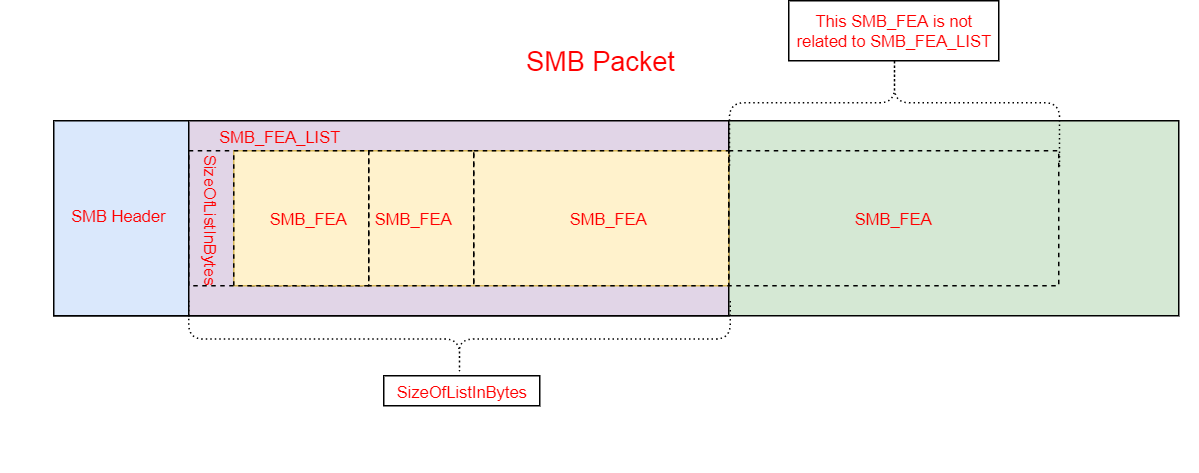
\includegraphics[width=15cm]{checkpoint_after_shrink_correct.png}
    \caption[FEAList nach korrekter Verkleinerung, Nadav Grossmann (Checkpoint Research), URL: \url{https://research.checkpoint.com/wp-content/uploads/2017/09/eternalblue5.png}]{Speicherbelegung der FEA Liste nach korrekter Verkleinerung}
    \label{img:fealist_after_shrinking_correctly}
\end{figure}

\begin{figure}[H]
    \centering
    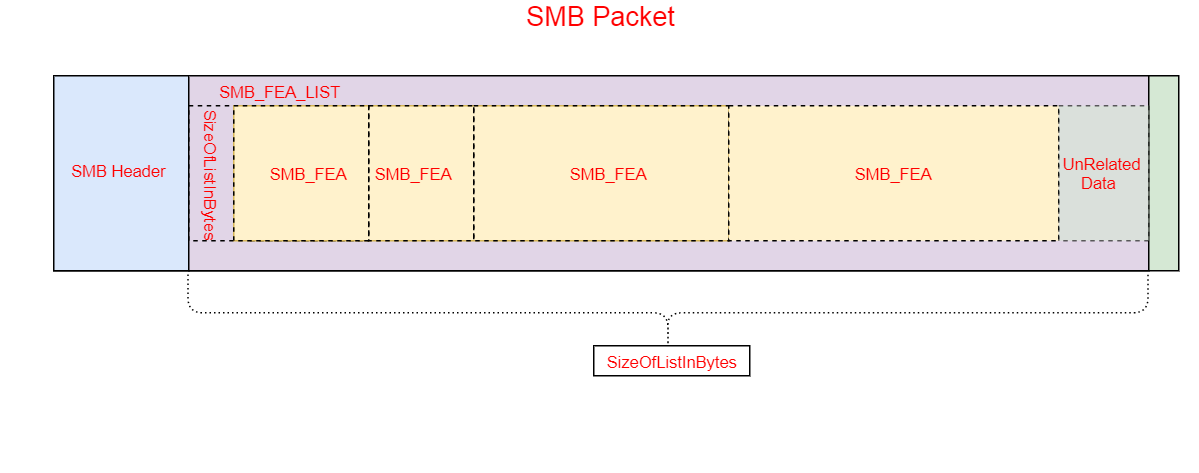
\includegraphics[width=15cm]{checkpoint_after_shrink_error.png}
    \caption[FEAList nach fehlerhafter Verkleinerung, Nadav Grossmann (Checkpoint Research), URL: \url{https://research.checkpoint.com/wp-content/uploads/2017/09/eternalblue6.png}]{Speicherbelegung der FEA Liste nach fehlerhafter Verkleinerung}
    \label{img:fealist_after_shrinking_incorrectly}
\end{figure}

\section{Falsches Parsen des SMB Datensegments}\label{sec:Wrong_Parse}
Für die Übertragung von Daten kommen zwei SMB Commands und deren Subcommands zum Einsatz, die für die Übertragung von Daten verantwortlich sind: \verb|SMB_COM_TRANSACTION2| und \verb|SMB_COM_NT_TRANSACT|. Durch Anhängen von \verb|_SECOND| kann jeweils der sekundäre Befehl gebildet werden \cite{MS:SMBCom}. Ist die in der Variable \verb|total_data_to_send| zu übertragende Datenmenge größer als die maximale in einem Paket sendbarew Größe, so werden die im primären Befehl noch ausstehenden Daten aufgeteilt und nach dem initialen Paket mittels des mit \verb|_SECONDARY| gebildeten Commands versendet, bis die zu übermittelnde Datenmenge vollständig sind\cite{TM:EB}.

\noindent
Die zwei Befehle samt deren Subcommands unterscheiden sich nur gering, aber in einem für den Exploit essentiellen Punkt signifikant, was für den erfolgreichen Hack von Bedeutung ist. Während \verb|SMB_COM_TRANSACTION2| die Bytegröße der zu sendenden Daten in einem Header Parameter in WORD-Größe abspeichert, nutzt \verb|SMB_COM_NT_TRANSACT| hierfür einen in DWORD-Größe. Das heißt, dass sehr große Parameterdaten gesendet werden können \cite{CP}.

\noindent
Ein weiterer wichtiger Faktor ist auch, dass nicht geprüft wird, mit welchem der beiden Befehle eine Transaktion gestartet wurde. Dieser Unterschied in der maximal adressierbaren Datenmenge der Transaktionsbefehlstypen und der Mangel an Validierung, ob der Transaktionsbefehl gleich bleibt, lassen sich für einen Angreifer ausnutzen, indem auf \verb|SMB_COM_NT_TRANSACT| ein \verb|SMB_COM_TRANSACTION2| gesendet wird\cite{SS:EB}. Das wiederum führt zum Auslesen der falschen Daten und ermöglicht somit fehlerhaftes Parsen durch Behandeln des WORD-großen Header Parameters in \verb|_TRANSACTION2| als DWORD, was die FEAs malformed und somit ungültig werden lässt\cite{CP}.

\section{Beliebige Allokation von Speicher im Non-Paged Memory Pool}\label{sec:MemAlloc}
Um eine Session beim Server über Port 445 aufbauen zu können, wird ein Authentifikationsrequest über die Funktion \verb|SMB_COM_SESSION_SETUP_ANDX| gesendet, was über IPC\$ einen anonymen User Logon beim Server etabliert und eine User ID kreiert \cite{MS:Auth}. Diese UID wird bei jeder der Transaktionen im SMB Header gesendet und ermöglicht das Zuordnen der Datenpakte zu einer Verbindung\cite{SS:EB}. Auch beim Etablieren des Logons gibt es wieder zwei unterschiedliche Formate, namentlich LM/NTLM und NTLMv2, auch bekannt als NTLM SSP. Diese besitzen bei eine ähnliche zweiteilige Struktur, welche aus zwei Blöcken, \verb|SMB_Parameters| und \verb|SMB_Data|, besteht \cite{MS:SMBCom}.

\noindent
\begin{minipage}{.45\textwidth}\label{LM/NTLM}
\begin{lstlisting}[language=C,caption={LM/NTLM Auth Request},captionpos=b]
SMB_Parameters
{
  //For this type of request
  //WordCount = 13
  UCHAR WordCount;
  Words
  {
    UCHAR AndXCommand;
    UCHAR AndXReserved;
    USHORT AndXOffset;
    USHORT MaxBufferSize;
    USHORT MaxMpxCount;
    USHORT VcNumber;
    ULONG SessionKey;
    USHORT OEMPasswordLen;
    ULONG Reserved;
    ULONG Capabilities;
  }
}
SMB_DATA
{
  USHORT ByteCount;
  Bytes{
    UCHAR OEMPassword[];
    UCHAR UnicodePassword[];
    UCHAR Pad[];
    SMB_STRING AccountName[];
    SMB_STRING PrimaryName[];
    SMB_STRING NativeOS[];
    SMB_STRING NativeLanMan[];
  }
}
\end{lstlisting}
\end{minipage}\hfill
\begin{minipage}{.45\textwidth}\label{NTLMv2}
\begin{lstlisting}[language=C,caption={NTLMv2 Auth Request},captionpos=b]
SMB_Parameters
{
  //for this type of request
  //WordCount = 12
  UCHAR WordCount;
  Words
  {
      UCHAR AndXCommand;
      UCHAR AndXReserved;
      USHORT AndXOffset;
      USHORT MaxBufferSize;
      USHORT MaxMpxCount;
      USHORT VcNumber;
      ULONG SessionKey;
      USHORT SecurityBlobLen;
      ULONG Reserved;
      ULONG Capabilities;
  }
}
SMB_DATA
{
  USHORT ByteCount;
  Bytes{
    UCHAR SecurityBlob[SecurityBlobLength];
    SMB_STRING NativeOS[];
    SMB_STRING NativeLanMan[];
  }
}
\end{lstlisting}
\end{minipage}
\hfill
\verb|SMB_Parameters| speichert in sich mehrere Parameter, die jeweils maximal vier Bytes an Speicher einnehmen können. Die Variable WordCount ist hier auch zu finden. Sie gibt die Länge der \verb|SMB_Parameters| Daten in WORDs an. Abhängig von Typ des Requests unterscheided sich auch deren Länge. Bei LM und NTLM beträgt diese stets 13 während die von NTLMv2 12 beträgt. Der zweite Teil beider Formate, \verb|SMB_Data|, beinhaltet Daten in unterschiedlicher Größe, wobei eine Variable namens ByteCount den benötigten Speicherplatz festhält\cite{CP}.
%In beiden Fällen führt der Server einen Integritätscheck mit einer Funktion namens SrvValidateSmb aus, um zu überprüfen, ob die Struktur eingehalten und unbeschädigt ist.
Wird ein Authentifikationsrequest als NTLMv2 ohne die Flag für ''Extended Security'' gesendet, wird folglich der Request fälschlicherweise als NTLM Request behandelt und in der Funktion, die den benötigten Speicherplatz berechnet, nicht die in ByteCount angegebene Größe der Daten, sondern die NativeOS und NativeLanMan Unicode Strings verwendet. Somit ist durch Manipulieren dieser Werte beliebig viel Speicher beim Verbindungsaufbau durch ein entsprechend modifiziertes Authentifikationsrequest allokierbar \cite{CP}.\\


\section{Ablauf}\label{sec:Ablauf}
Eine von einer Anzahl an Möglichkeiten, die oben beschriebenen Methoden auszunutzen, ist, SMBv1-Verbindungen,und SMBv2 Verbindungen in Kombination miteinander zu verwenden. Hierbei muss durch entsprechendes Legen der Speicherblöcke wie unter \ref{sec:Grooming} beschrieben eine Konstellation entstehen, bei der ein durch SMBv2 genutzter Speicherblock hinter einem durch SMBv1 entstandenen Chunk platziert wird. Durch den unter \ref{sec:FEA_Cast} beschriebenen Overflow, der durch die fehlerhaften FEAs wie in \ref{sec:Wrong_Parse} ermöglicht wird, können beliebige Daten in den Headerbereich des SMBv2 Speicherblocks geschrieben werden, welcher auf die nächste Position von zusammengehörigem Speicher verweist. Sobald das nächste Paket der SMBv2 Transaktion in den Speicher geladen werden soll, wird der Inhalt an die manipulierte Speicheradresse geschrieben. Durch Überschreiben von diesem Pointer kann somit über SMBv2 gesendeter Schadcode zum Beispiel in den HAL geladen werden. Im Header existiert ein weiterer Pointer, der eine Handler Methode beim Schließen der Verbindung aufruft\cite{CP}. Durch das Hinterlegen der Speicheradresse des Schadcodes kann beim Schließen der SMBv2 Verbindung dieser aufgerufen werden, womit die Remote Code Execution abgeschlossen ist\cite{SS:EB}.


\chapter{Prävention und Schutz}
Wie bei den meisten anderen Softwareproblemen empfielt sich, regelmäßig Updates aufzuspielen, um Sicherheitslücken durch Patches zu schließen. Das Update, das Hacking mittels des EternalBlue Exploits verhindert, ist seit März 2017 für alle relevanten Windows Produkte verfügbar.
Da der Exploit eine ganze Kette an Bugs benötigt, die zusammen arbeiten, um einen erfolgreichen Hack durchzuführen, reichte es aus, dass der Typ von SizeOfListInBytes zu DWORD geändert wurde\cite{Scad:EB}, da hierdurch beim Reduzieren der Listengröße alle stellen der Zahl geupdated werden.
Um zu überprüfen, ob eine Maschine die Sicherheitslücke noch aufweist, hat die Firma Sophos ein Powershell-Skript bereit gestellt, welches auf Windowsversion, Betriebssystem und Updates prüft, um anschließend die Verwundbarkeit auszuwerten\cite{SAV}.\\
Neuere Windows 10 und Windows Server Installationen werden ab dem Fall Creators Update 2017 auch nicht mehr standardmäßig die seit 2014 offiziell als veraltet geltende SMBv1 Schnittstelle installiert haben. Sollte das Protokoll für Legacy Geräte noch benötigt werden, kann es aber jederzeit über die Windows-Features wieder installiert werden \cite{MS:Fix}.\\
Da das SMBv1-Protokoll als relativ unsicher gilt und hauptsächlich für die Unterstützung alter Systeme benötigt wird, kann es auf den meisten Rechnern ohne negative Folgen deaktiviert bzw. deinstalliert werden \cite{WP}, da die neueren, üblicherweise bei der Installation schon akivierten SMB Versionen  seit einiger Zeit der neue Standard sind und mehr Funktionen aufweisen. Das kann zum Beispiel unter Windows 10 über die Funktion ''Windows-Features'' der Systemsteuerung gemacht werden. Es gilt seit jeher, dass Systemadministratoren in großen Netzwerken unbenutzte Ports stets geschlossen halten und obsolete und oder ungenutzte Protokolle deaktivieren sollten.\cite{TM:EB}

\chapter{Fazit}
Wieder einmal zeigt ein Exploit auf, wie gefährlich in die Jahre gekommener Legacy Code auch für moderne Systeme sein kann. Besonders in einer Zeit, in der Regierungen solche Sicherheitslücken gezielt suchen und sammeln, um eine Art Rüstungskrieg mit dem Rest der Welt zu führen.\\
Der entstandene Schaden in Milliardenhöhe sollte vielen Entwicklern, besonders im Bereich der Netzwerkprotokolle, ein Ansporn sein, sauberen Code zu schreiben und diesen auch auf so obskure Kombinationen wie enorme über 64kB große Pakete oder falsch geflaggte Requests zu testen. Dass der falsche Umgang mit einer Zahl in knapp 30 Jahre altem kaum noch genutzem Code ein so verheerendes Chaos anrichten kann, lässt erahnen, welche gravierenden Sicherheitlücken, so unscheinbar sie auch sein mögen, in Zukunft noch entdeckt oder bereits unter strenger Geheimhaltung ausgenutzt werden. Für's erste jedoch scheint durch Bemühungen Microsofts und vieler Systemadministratoren der Gefahrenherd, den das SMBv1 Protokoll darstellt, Geschichte zu sein.

\clearpage
\label{sec:sources}
\renewcommand{\bibname}{Quellenverzeichnis}
\bibliographystyle{unsrtdin}
\bibliography{itsec}
\addcontentsline{toc}{chapter}{Quellen- und Literaturverzeichnis}

\end{document}